\documentclass[12pt,titlepage,french]{article}
\usepackage{babel}
\usepackage{graphicx}
\usepackage[margin=2.5cm]{geometry}

\usepackage[hidelinks]{hyperref}
\usepackage{tabularx}
\usepackage[utf8]{inputenc}
\usepackage[T1]{fontenc}
\pagestyle{plain}

\usepackage{booktabs,makecell,tabu}
\usepackage{comment}
\renewcommand\theadfont{\bfseries}

\linespread{1.5}

\newcounter{firstbib}

\begin{document}
%\renewcommand{\thesection}{\arabic{section}} % utilisé pour spécifier la numérotation des sections

\begin{titlepage}
\newcommand{\HRule}{\rule{\linewidth}{0.5mm}}
\center

  
\includegraphics[width=0.45\textwidth]{../../ressources/img_logos/logo_polytech.png}\\[1cm]

  
\includegraphics[width=0.45\textwidth]{../../ressources/img_logos/logo_taglabs.png}


\HRule \\[0.4cm]
{ \huge \bfseries Rapport itération 3\\[0.15cm] }
Classification colorimétrique de nuages de points 3D\\
Version 1.1\\
Le \today \\
\HRule \\[1.5cm]
Ronan Collier,
Mathieu Letrone,
Tri-Thien Truong
\\[1cm]
\end{titlepage}

\tableofcontents % table des matières
\newpage
\listoffigures  % table des figures
\newpage

\section{Rappel des objectifs de l'itération}
Pour cette itération, nos objectifs étaient surtout concentrés sur l'amélioration de notre solution existante. En effet, Nous avions réussi à créer un plugin sur le logiciel CloudCompare, en se basant sur le plugin existant "QPCL". Toutefois, nous voulions exporter notre projet sur un plugin à part, afin de rendre le code plus facile à maintenir, et de bien distinguer ce que nous dévelopions, à ce qui était déjà présent.

Les tâches que nous nous sommes fixées sont les suivantes :

\begin{itemize}
  \item Refactoring du code / Exportation sur un nouveau Plugin
  \item Amélioration de la sélection de points dans le nuage
  \item Amélioration du filtrage RGB / Conversion LAB
  \item Intégration du Point picking, du filtrage multi-scans
\end{itemize}

\section{Production / réalisation durant l'itération}

Nous déveloperons ici chaque objectif que nous nous sommes fixé pour cette itération.

\subsection{Refactoring du code / Exportation sur un nouveau Plugin}

Nous avons pris le temps pour revoir notre structure du code, afin de l'exporter sur notre propre projet. Pour faire cela, nous nous sommes basé sur un template de plugin CloudCompare, disponible sur le git du projet. \newline

Ensuite, nous avons repris notre code développé sur le plugin QPCL, pour le mettre sur notre nouveau projet. Pour faire cela, nous avons dû enlever les dépendances avec QPCL (donc les méthodes de la bibliothèques PCL pour traiter des nuages de points). Nous avons donc utilisé uniquement les outils intégrés à CloudCompare, pour faire nos traitements. \newline

Nous aurions pu créer une dépendance avec le plugin QPCL, et notre propre plugin, mais nous voulions d'abord voir s'il était possible de faire nos filtrages / segmentation avec les outils de CloudCompare, ce qui était effectivement le cas. Pour voir si notre choix était le bon, nous avons comparé notre ancienne méthode (utiliser la bibliothèque de PCL), et la nouvelle (uniquement CloudCompare). Le critère de comparaison a été au niveau du temps pour réaliser notre filtrage (RGB). \newline

Nous avons réalisé des tableaux comparatifs entre notre ancienne méthode d'implémentation (avec QPCL), et notre nouvelle implémentation (CloudCompare CC). \newline

\begin{figure}[!hbtp]
  \caption{\label{} Nuage de points de test}
  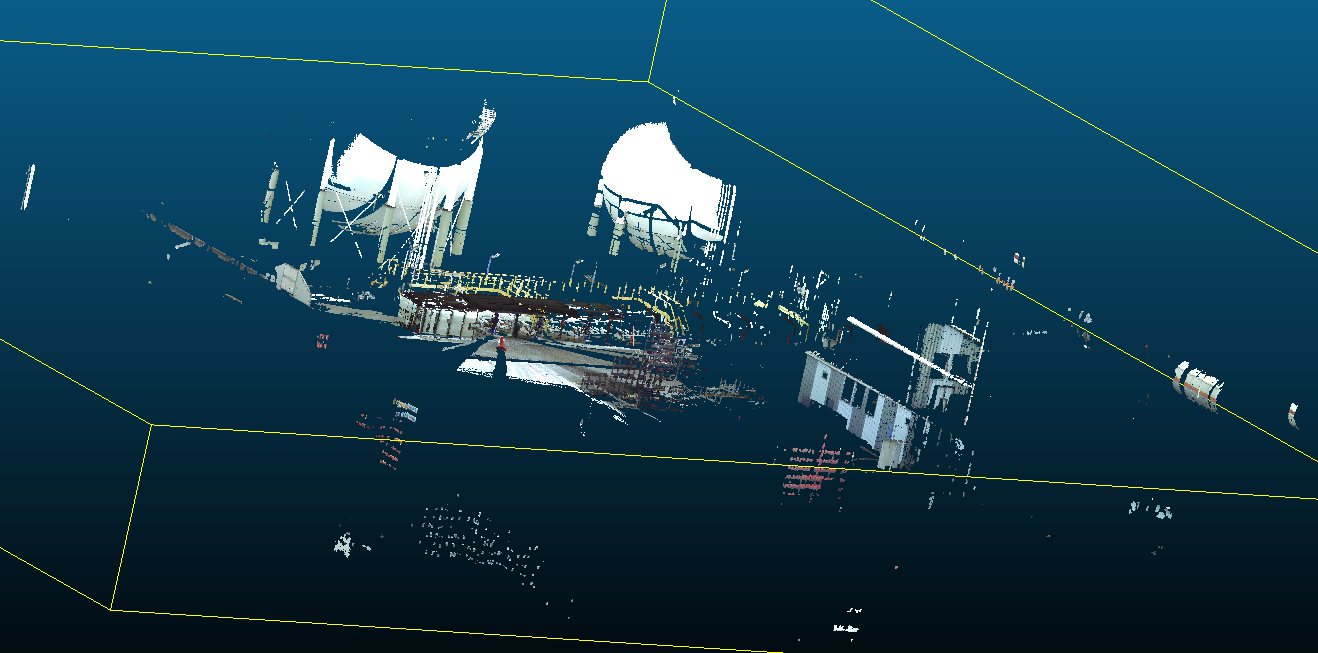
\includegraphics[width=1\textwidth]{./img/scan.png}
\end{figure}

Le fichier de test contient 22 649 423 points. Nous avons décidé de choisir un fichier très volumineux, puisque dans une situation réelle, tous les nuages de points seront aussi volumineux. Notre algorithme devra donc s'adapter à ce genre de jeu de données. De plus, les tests réalisés sur des nuages de points plus petits (de l'ordre de 100 x plus petit) apportaient des résultats très similaires, donc la comparaison n'était pas très représentative. \newline

\begin{figure}[!hbtp]
  \caption{\label{} Relevés des temps QPCL et CC}
  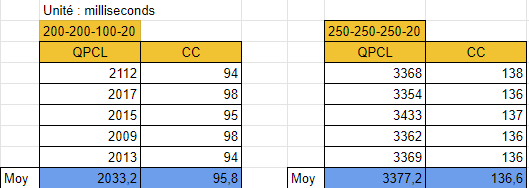
\includegraphics[width=1\textwidth]{./img/donnees.png}
\end{figure}

Nous pouvons voir dans la figure 2, les valeurs de temps, en millisecondes, relevées sur notre filtrage RGB du nuage de points de la figure 1. Le tableau de gauche permet de faire un filtrage sur les points de couleur jaunâtre (RGB : 200 - 200 - 100), avec une marge d'erreur de 20\%.

Pour comparer avec un filtrage où il y a un grand nombre de points à garder, nous avons fait un autre filtrage avec les points de couleur blanc (250 - 250 - 250, marge d'erreur de 20\%). \newline

Nous observons qu'il y a une grande différence entre les deux méthodes. Le filtrage avec des méthodes de CloudCompare uniquement, est beaucoup plus rapide qu'en utilisant QPCL. Notre deuxième méthode est de l'ordre d'environ 20 fois plus rapide que notre ancienne méthode. Nous avons donc un gain de temps énorme sur notre nouvelle méthode. \newline

Cela est probablement dû au fait qu'avant, nous utilisions une conversion du nuage de points d'un objet avec CloudCompare, en objet de PCL. Ensuite, nous réalisions le filtre avec ce type de nuage, pour ensuite reconvertir le nuage filtré en un objet CloudCompare, pour finalement l'afficher. Ces différentes étapes n'existent plus sur notre nouveau filtrage.

\subsection{Amélioration de la sélection de points dans le nuage}
Jusqu'à présent la segmentation du nuage de point n'était qu'on simple filtrage des points par rapport à une valeur RGB de référence.
Il s'agit d'une méthode répondant au besoin mais qui n'en demeure pas moins simpliste et manquant d'éfficacité.
Lors de nos recherches réalisées dans le cadre de la première itération, nous avons aboutit à la découverte du'ne nouvelle méthodes de segmentation colorimétrique \cite{B01}.
Cette 3ème itération devait permettre l'implémentation de ce nouvel algorithme.
Cependant, les ajouts de nouvelles tâches ainsi que les imprévus nous ont freinés dans son implémentation.
La segmentation est donc à l'heure actuelle dans un état embryonnaire.
Seule la structuration de bases des méthodes est présente.
% Nouvel algo en cours, expliquer où ça en est, ce qui reste à faire...
%TODO : Ronan

\subsection{Amélioration du filtrage RGB / Conversion LAB}

Suite aux retours de notre client, nous avons pu revoir l'utilisation du filtrage RGB implémenté lors de notre précédente itération. Une des propositions était d'utiliser qu'un seul point à choisir pour appliquer le filtrage RGB, et de la marge d'erreur pour établir les bornes des points à garder. \newline

\begin{figure}[!hbtp]
  \caption{\label{} Ancienne interface et nouvelle interface filtrage RGB}
  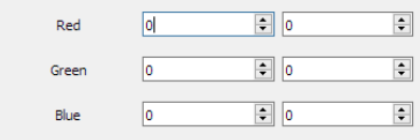
\includegraphics[width=0.4\textwidth]{./img/rgb_old.png}
\hspace*{1in}
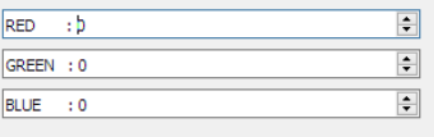
\includegraphics[width=0.4\textwidth]{./img/rgb_new.png}
\end{figure}

A gauche, nous pouvons observer l'ancienne interface (uniquement les champs pour le RGB), et à droite, la nouvelle interface. \newline

Suite à notre réunion de fin d'itération, l'idée de la sélection de deux points est plus intéressante au final, puisque cela nous permettra de sélectionner des bornes plus facilement. En effet, dans un nuage de points, d'un objet d'une certaine couleur peut avoir beaucoup de variation au niveau de cette couleur, selon l'endroit d'où il est pris par la station, la luminosité etc. \newline

La conséquence est donc le fait que les valeurs RGB des points peuvent énormément variées, malgré le fait que visuellement, nous avons la même couleur. En gardant la sélection de deux points, nous pourrons donc définir des bornes minimum et maximum des valeurs RGB, au lieu de faire varier la marge d'erreur, qui n'est pas forcément très pertinent sur notre problème.

% Conversion LAB, but de cette conversion, comment ca fonctionne, résultat obtenu, conclusion sur son utilisation
% TODO : Mathieu

\subsection{Intégration du Point picking, multi-scans}

% Idée du point picking, le pourquoi, fonctionnement, pertinence pour le projet
% TODO : Thien

% Idem pour Multi-scans

\section{Risques éliminés durant l'itération}
Durant cette itération, nous avons pu éliminer certains risques. En effet, le fait d'utiliser uniquement les outils de CloudCompare nous permet d'éviter d'être dépendant de la bibliothèque PCL. \newline

Bien sûr, il sera peut être possible dans le futur, que nous aurions besoin d'utiliser cette biliothèque pour certaines fonctions (par exemple, l'algorithme permettant de supprimer les points isolés). Mais pour l'instant, traiter les nuages de points avec le code que nous fournis CloudCompare nous suffit, et nous apporte un gain de temps non négligeable. \newline

Nous avions aussi des interrogations par rapport à notre méthode d'implémentation de notre plugin. En effet, le fait d'avoir notre propre plugin est une amélioration très importante quant à notre projet, puisque nous avons uniquement des fichiers qui servent au fonctionnement de notre plugin. L'implémentation est donc beaucoup plus aisée.

\section{Commentaires sur l'itération}

\subsection{Commentaires sur l'itération de façon générale}

\subsection{Commentaires sur les méthodes de travail/changements de méthode}

\section{Trois principaux risques restants}


\section{Objectifs de la prochaine itération}

Durant cette itération, nous avons pu grandement mettre en ordre notre projet. Nous avons donc maintenant notre propre plugin. Il faut maintenant terminer ce qui était en cours, prendre en compte les retours du client, et continuer les tâches prévues du cahier des charges.

Les tâches prévues sont donc les suivantes :

\begin{itemize}
  \item Intégration de fausses couleurs
  \item Terminer la nouvelle méthode de segmentation
  \item 
\end{itemize}

\begin{comment}

\section{Résumé}
\subsection{Tâches principales réalisées dans l'itération}
\noindent\begin{tabu} to \textwidth {p{0.18\textwidth}X[c2]X[c]X[c4]}\toprule
  \thead{Tâche}&\thead{Responsable}&\thead{Statut}&\thead{Commentaire}\\\toprule
Plugin pour CloudCompare
& Mathieu
& Achevé
& Plugin CloudCompare possible, ou développer une interface à la main. Le choix est de faire un plugin CloudCompare.\\\midrule
Bibliothèques pour le traitement de nuages de points
& Ronan, Tri-Thien
& Achevé
& PCL semble la bibliothèque principale à utiliser, par sa simplicité et toutes les fonctionnalités qu'elle peut nous fournir.\\\midrule
Choix du langage
& Tri-Thien
& Achevé
& C++ ou Python. Le choix est le C++ pour faciliter l'implémentation du code avec CloudCompare. \\\midrule
Architecture du code source
& Ronan, Tri-Thien, Mathieu
& Achevé
& Organisation avec un package pour le plugin CloudCompare, et un autre pour nos algorithmes.\\\midrule
Espaces colorimétriques
& Mathieu
& Achevé
& Le format RGB est le plus répendu, mais l'option du CIELab semble être intéressant.\\\midrule
Algorithmes de segmentation
& Ronan, Tri-Thien, Mathieu
& Achevé
& Méthode pour segmenter selon une couleur (et un seuil d'erreur). Autre alternative : classification des points et régions puis raffinement\\\midrule
Recherche sur les méthodes de fausses couleurs
& Ronan
& Achevé
& Correspondre une valeur en intensité en RGB (ou autre). Création d'une palette de couleurs.\\\bottomrule  \\
\end{tabu}

\subsection{Tâches principales à réaliser pour la prochaine itération}
\begin{itemize}
  \item Plugin CloudCompare
  \item Développer la sélection de points selon une couleur définie
  \item Développer une solution pour extraire des points dans le nuage
  \item Mettre le code en commun.
\end{itemize}

\end{comment}

\begin{thebibliography}{3}

\bibitem{B01} Qingming Zhan, Yubin Liang, Yinghui Xiao, \textit{Color-based segmentation of point clouds}, 2009
\end{thebibliography}
\end{document}
